\documentclass{JoITSRstyle}
\usepackage{graphicx}
\usepackage{times}
%\usepackage{epsfig}
%\usepackage{graphicx}
\usepackage{amsmath}
\usepackage{amssymb}
\usepackage{subfigure}
\usepackage{color}
\usepackage%[usenames,dvipsnames]
{xcolor}
%\usepackage{algorithm}
%\usepackage{algorithmic}
\usepackage{authblk}
\usepackage{abstract}
\usepackage{comment}
%\usepackage{wrapfig}
\usepackage[normalem]{ulem}
\usepackage{url}
\renewcommand\Authands{, }



\begin{document}
\title{Detection of Emergency Telephone Indicators in a Tunnel Environment}

\author[1]{Zhipeng Wang}
\author[1]{Matasaka Kagesawa}
\author[1]{Shintaro Ono}
\author[2]{Atsuhiko Banno}
\author[1]{Takeshi Oishi}
\author[1]{ and\\Katsushi Ikeuchi}

\affil[1]{Institute of Industrial Science, The University of Tokyo, Japan \authorcr
Email: \{wangzp,kagesawa,onoshin,oishi,ki\}@cvl.iis.u-tokyo.ac.jp}
\affil[2]{Advanced Industrial Science and Technology, Ibaraki, Japan  \authorcr
Email: atsuhiko.banno@aist.go.jp}
\twocolumn[
\begin{@twocolumnfalse}
\maketitle
{\normalsize
Positioning of vehicles is important for ITS. In a tunnel environment, most positioning solutions based on GPS sensors or ordinary cameras will fail. For positioning we propose a method to detect emergency telephone indicators in a tunnel environment by using infrared cameras. The proposed detection method makes use of both appearance and motion information of the target objects. By optimizing the detecting pipeline, the method works in real time and produced 100\% detection rate and 0\% false alarm rate in one of our experiments. }

\begin{center}
\emph{\textbf{Keywords: }Object detection, Positioning}
\end{center}
\emph{}
\\
\end{@twocolumnfalse}
]



\section{Introduction}
% no \IEEEPARstart
Positioning of vehicles acts as a fundamental role in autonomous driving, and is also of great importance for driving assistance, vehicle navigation, etc. When GPS sensors function properly, the task is easy. While in a tunnel environment, there are no GPS signals available for most of the time. A new positioning system which functions properly in a tunnel environment is necessary~\cite{nig}. In this paper we propose an object detection method which can be used for positioning systems in tunnels.

Our proposal is part of an automated driving system in a NEDO project, "Development of Energy-saving ITS Technologies".
{\color{red} The automated driving system is vehicle-oriented, and an express way is the main application scenario. No specific facilities are assumed to exist on road sides, while instead, the experimental vehicles are equipped with  sensors and vehicle-to-vehicle communication systems. There are a few sensors used for positioning. For example, sensors used to extract white road lines to estimate the lateral position in the lane, GPS sensors, dead reckoning systems, and stereo far-infrared camera systems intended for obstacle detection. On the street, GPS sensors can be used for positioning. While positioning in tunnels is difficult since GPS signals are not available and no specific equipment on road sides is assumed. For positioning in tunnels, GPS sensors are used to record the position of  tunnel entrances, and dead reckoning systems are used to infer position by continuously sensing the vehicles' speed and direction. However, errors of dead reckoning systems will accumulate. Thus, the proposed method uses far-infrared cameras installed on the vehicles to detect signs in the tunnels, which contain position information, and will be used to eliminate the accumulated errors. }

\begin{comment}
{\color{red}For automatic driving, positioning is very important, and current positioning methods in tunnels often have the problem of accumulated errors. These methods usually rely on the initial position at the entrance of a tunnel obtained from a GPS signal, and the continuous recording of automobile status, i.e. speed and direction of the vehicle. It is obvious that the errors will accumulate. If some signs with position information can be detected while going through the tunnel, the problem of accumulated errors can be solved.}
\end{comment}

In most tunnels   on the expressways in Japan, there are many signs appearing at equal intervals. We focus on the emergency telephone indicators, which appear every 200 meters in tunnels. The absolute coordinates of the emergency telephone indicators can be obtained by the method of~\cite{xue}.  If the emergency telephone indicators can be sensed while traveling in tunnels, and the distance from the vehicle to the indicators can be estimated,  then this information  can be used to eliminate accumulated errors of dead reckoning systems.
Detection methods, e.g.~\cite{ac23}, based on ordinary cameras fail due to darkness. Here we use far-infrared cameras,  which are suitable in dark environments and are already installed on our experimental vehicles. Inspired by a previous work~\cite{wang1}, we propose an approach to detect emergency telephone indicators.




Detection performance and efficiency are the two important aspects of our method.
In a tunnel environment, in addition to the target objects, a lot of noisy objects also appear, e.g. ordinary lights, other vehicles, and other vehicles' shadows. And some of the noisy objects cannot even be distinguished from the target objects by appearance , as shown in Figure \ref{fig:first}. The clutter property of the sensed data makes the detection challenging.
Our method meets this challenge by making use of both appearance and temporal information of the target objects. There are two main steps in the method. The first step deals with keypoints. It takes original data as input, and outputs keypoint clusters as detection hypotheses. In this step, keypoints are detected, verified and then clustered. To detect keypoints, all points on each frame are uniformly sampled and filtered with pre-set intensity thresholds.  Then the keypoints are verified by a simple keypoint appearance model   built by \emph{k}-means. At the end of the first step, the keypoints are clustered based on the Euclidean distance. The second step takes the keypoint clusters as input, verifies them by appearance and temporal information, and outputs the keypoints which pass verification, as detection results. In the second step, the keypoint clusters are labeled based on appearance by an Adaboost machine, which is trained using intensity histograms of keypoint clusters from target objects and keypoint clusters from noisy objects. The keypoint clusters are also tracked by temporal association through frames. Motion information encoded in the trajectories are used to further verify the keypoint clusters. Finally, the keypoint clusters which pass both appearance and temporal verifications are confirmed as emergency telephone indicators.

This pipeline is also designed  with consideration for the requirement of efficiency.  The method deals with the large amounts of information contained on one frame, following a hierarchical manner. The later a step is, the more time-consuming it is, and the fewer instances it deals with. From an image containing $10^5$ pixels, $10^4$ points go through the keypoint detection step of testing by intensity thresholds. Then in average, $10^3$ keypoints are detected, and verified, leaving about $10^2$ keypoints to be clustered. Afterwards, fewer than $10$ keypoint clusters are left; these are dealt with by the very time-consuming steps of generating image features and tracking.





\begin{figure}
\centering
\subfigure[]{
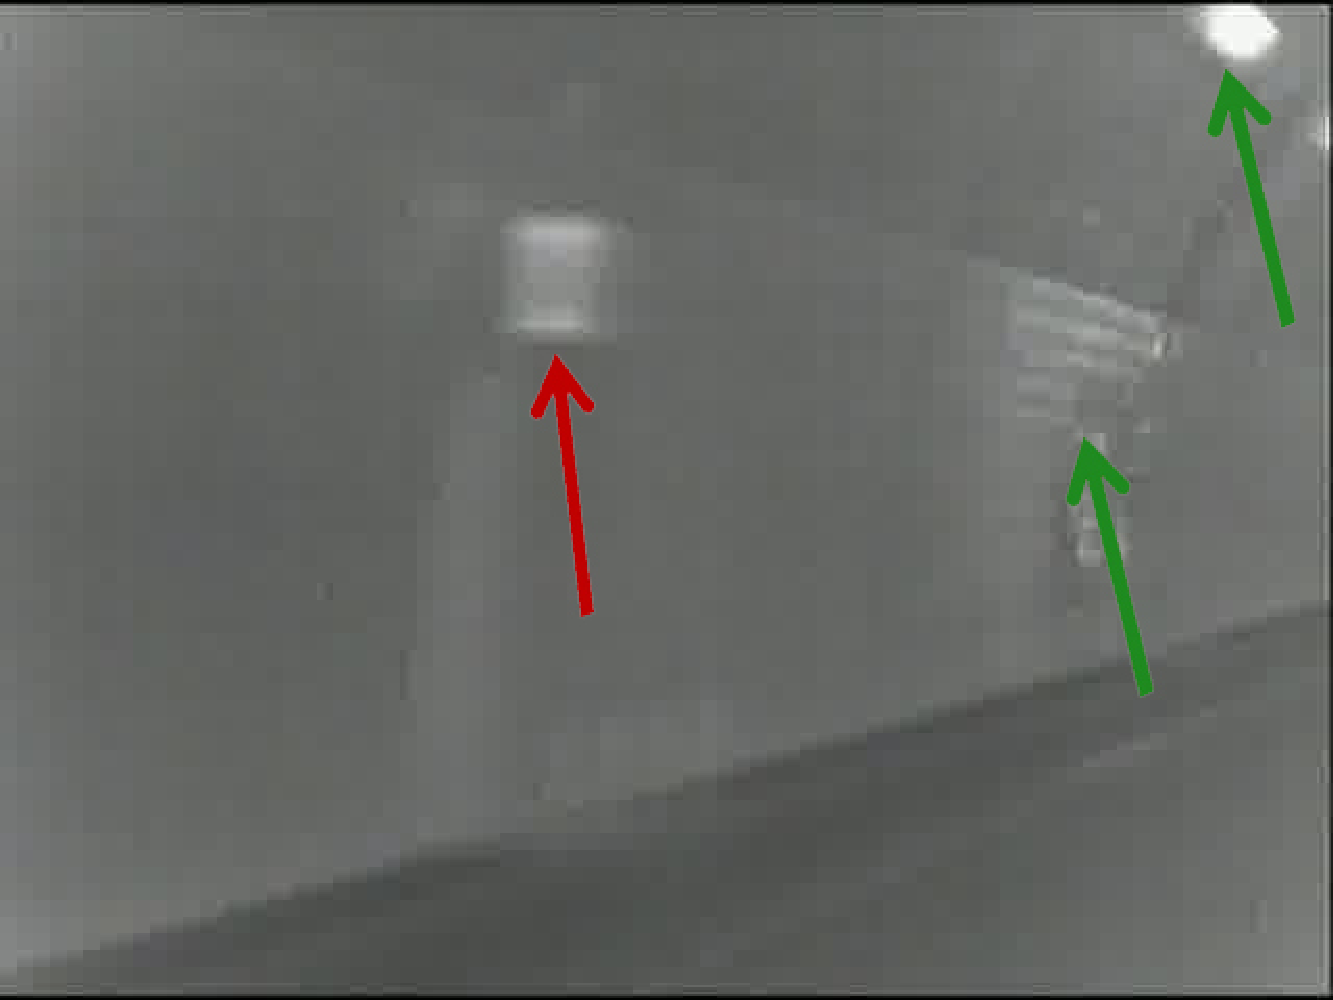
\includegraphics[width=0.22\textwidth,bb=0 0 640 480]{17Orgimg00039.ps}
\label{fig:first:a}}
\subfigure[]{
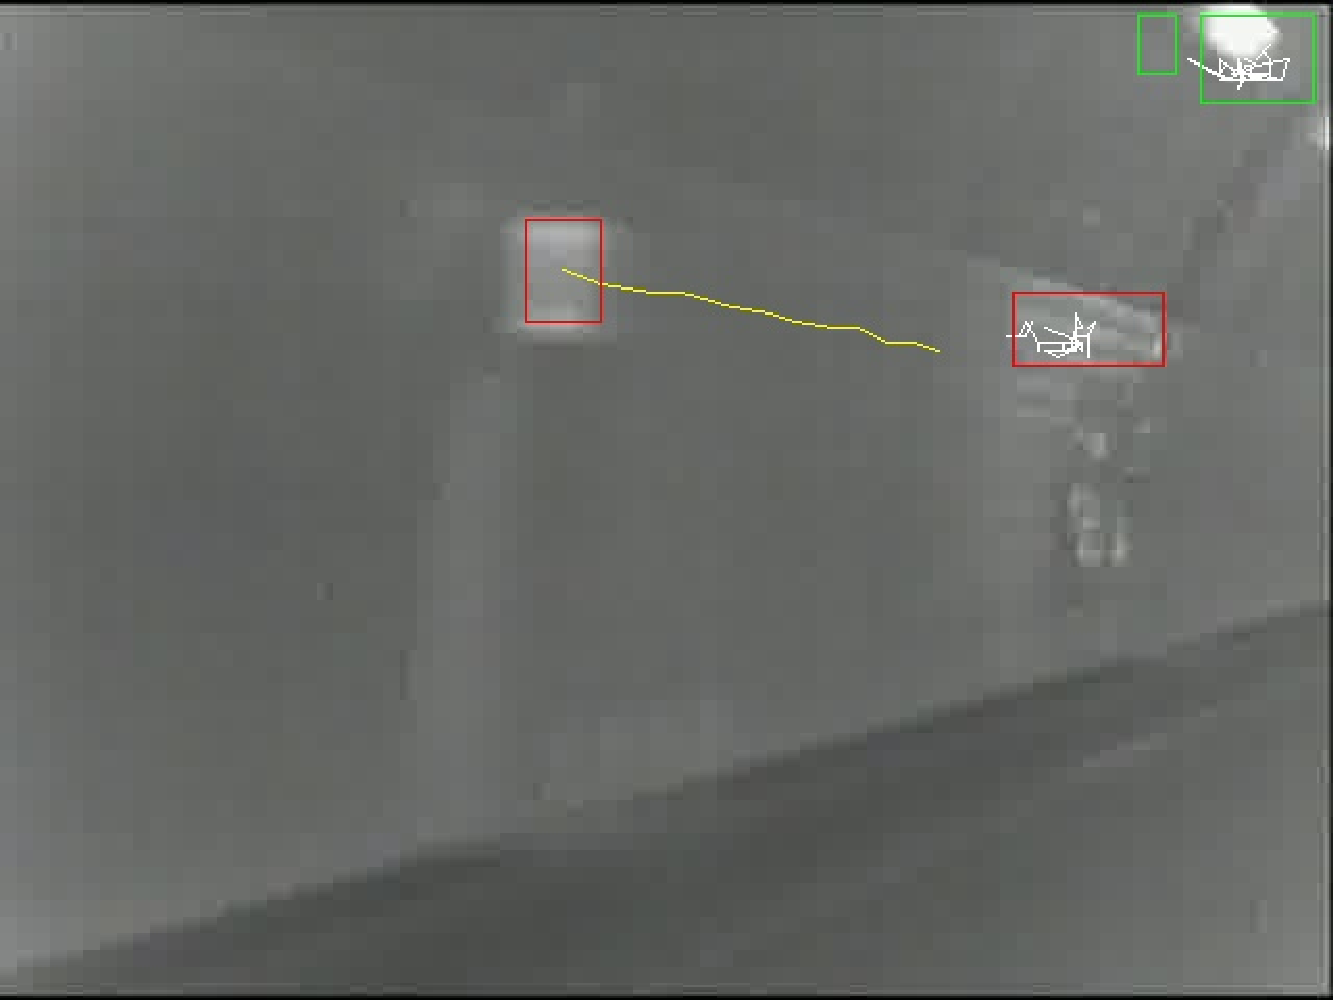
\includegraphics[width=0.22\textwidth,bb=0 0 640 480]{17veriTrjimg00039.ps}
\label{fig:first:b}}
\caption{Original data and detection results. In (a), the red arrow points to the target object: emergency telephone indicator, and the green arrows point to noisy objects. In (b), red rectangles mark detection hypotheses labeled as positive using appearance information, and green rectangles mark negative ones. Yellow trajectories mark detection hypotheses labeled as positive using temporal information, and white trajectories mark negative ones.}
\label{fig:first}
\end{figure}







The advantage of our method is its ability to give promising detection results from cluttered data in real time. In addition, this method successfully  combines bottom-up and classification methods, as well as combines both appearance and temporal information.

The paper is organized as follows: section 2 reviews related work, section 3 proposes a pipeline for the method, section 4 gives experimental results, and section 5 concludes.

\section{Related Work}


Most modern detection methods fall into two categories. Some~\cite{ij4,ac31,ac30,ac4,ac32,ac29,ac28,ac1} follow the sliding-window schema, and they detect objects by considering whether each of the sub-images contains an instance of the target object. Classifiers are usually employed by these methods. The other methods~\cite{ac9,ac2,ac3,ac5,ac10,ac21,ac18} infer object centers based on local image features in a bottom-up manner. The proposed method takes advantages of both frameworks. Following the bottom-up manner, keypoints are detected, verified, and clustered. After these steps, the keypoint clusters are considered as detection hypotheses. Then following the sliding-window schema, the keypoint clusters are verified by their appearance and temporal information, using discriminative methods.
Previous methods~\cite{ac34} also consider the combination of the two frameworks. Detection hypotheses are gained using a Hough transform and then verified by support vector machines in~\cite{ac10,ac25}. The methods in~\cite{ac6,ac7}, use randomized decision trees for both decisions: whether local features belong to foreground objects or not, and decisions of their Hough votes. The method proposed in~\cite{ac27} describes both frameworks in the same manner. While giving state-of-the-art detection performance, these other methods can't meet the requirement for efficiency as our method does.
Our work is also related to feature grouping methods~\cite{ac25}, detecting methods using trajectories~\cite{my9,ac24}, tracking methods~\cite{my7,my10}, and methods integrating appearance and temporal information~\cite{ac23}.
Especially, compared with the method proposed in~\cite{wang1}, our method employs a more effective classifying machine by setting biased weights for positive and negative training examples, and far over-performs~\cite{wang1}.

\section{Emergency Telephone Indicator Detection}
Our proposal can be considered a two-step method. The first step deals with keypoints. It
takes original data as input, and outputs keypoint clusters as detection hypotheses. The second
step takes these keypoint clusters as input, verifies them by their appearance and motion
information, and outputs the ones which pass verifications as detection results.

\subsection{Keypoint Detection}
In data collected using ordinary cameras, keypoints~\cite{o2,o12} invariant to rotations, affine changes, and illumination changes are preferable. In our case, keypoint detection is intended to provide hypotheses for emergency telephone indicators. Thus intensity is of great importance. Our method employs a simple yet useful method to detect keypoints. Firstly, points are uniformly sampled for an offset of 6 in width, and 7 in height (the length of an emergency telephone indicator is larger than its width). In this manner the magnitude of instances is reduced by nearly two orders. Then points that pass the test, which verifies them by setting intensity thresholds, are considered as keypoints.
Here a Gaussian distribution is assumed for the intensities of the points.


let$\{\bf{x}\}$ denote all the sampled points, $I_{\bf{x}}$ the intensity of each point, \begin{comment}$I_{\bf{x}}\sim{\mathcal{N}(\mu_{I_{\bf{x}}},{\sigma_{I_{\bf{x}}}}^2)}$,
\end{comment}
and $l_{\bf{x}}$ the label. If the point is considered as belonging to emergency telephone indicators, $l_{\bf{x}}=1$, otherwise, $l_{\bf{x}}=0$. By setting lower threshold, $I^{th1}_{\bf{x}}$,  and higher threshold, $I^{th2}_{\bf{x}}$, the probability that points belongs to emergency telephone indicators based on their falling into this interval is given by,
\begin{equation}
P(l_{\bf{x}}=1|I^{th1}_{\bf{x}}{\leq}I_x{\leq}{I^{th2}_{\bf{x}}})=
\frac
{P(l_{\bf{x}}=1,I^{th1}_{\bf{x}}{\leq}I_x{\leq}{I^{th2}_{\bf{x}}})} {P(I^{th1}_{\bf{x}}{\leq}I_x{\leq}{I^{th2}_{\bf{x}}})}\;.
\label{eq1}
\end{equation}

At this step, the possibility that as few points as possible, belonging to the emergency telephone indicators, are excluded, is also considered. The probability of one point falling into the defined interval based on its belonging to emergency telephone indicators is given by,
\begin{equation}
P(I^{th1}_{\bf{x}}{\leq}I_x{\leq}{I^{th2}_{\bf{x}}}|l_{\bf{x}}=1)=
\frac
{P(l_{\bf{x}}=1,I^{th1}_{\bf{x}}{\leq}I_x{\leq}{I^{th2}_{\bf{x}}})} {P(l_{\bf{x}}=1)}\;.
\label{eq1.1}
\end{equation}

Points for which the intensities fall in the pre-set thresholds, are detected as keypoints.
\begin{figure}
\centering
\subfigure[]{
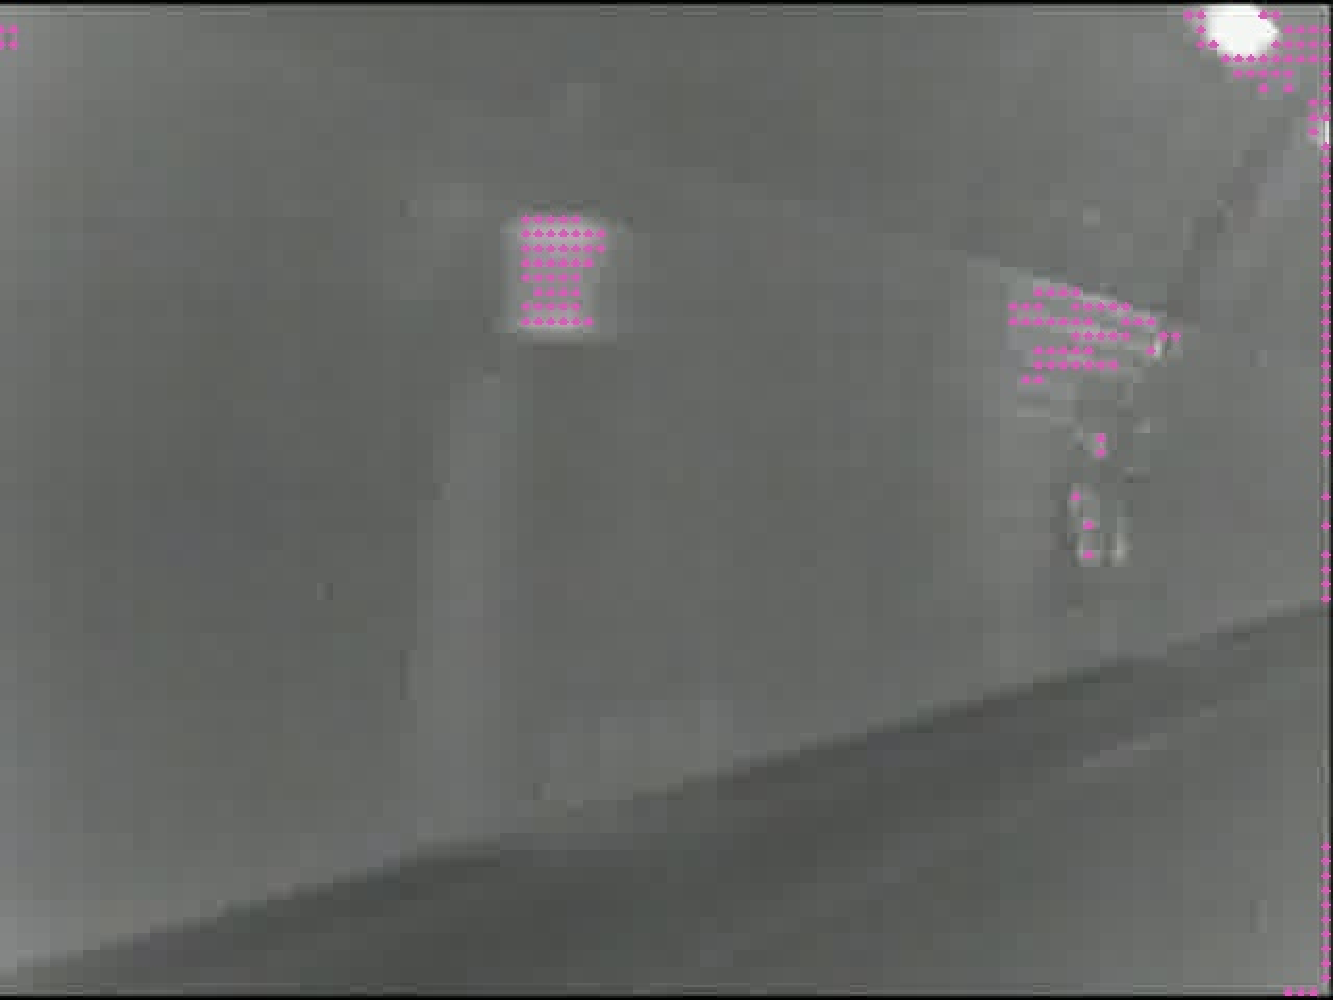
\includegraphics[width=0.22\textwidth,bb=0 0 640 480]{17Kptimg00039.ps}
\label{fig:sec:a}}
\subfigure[]{
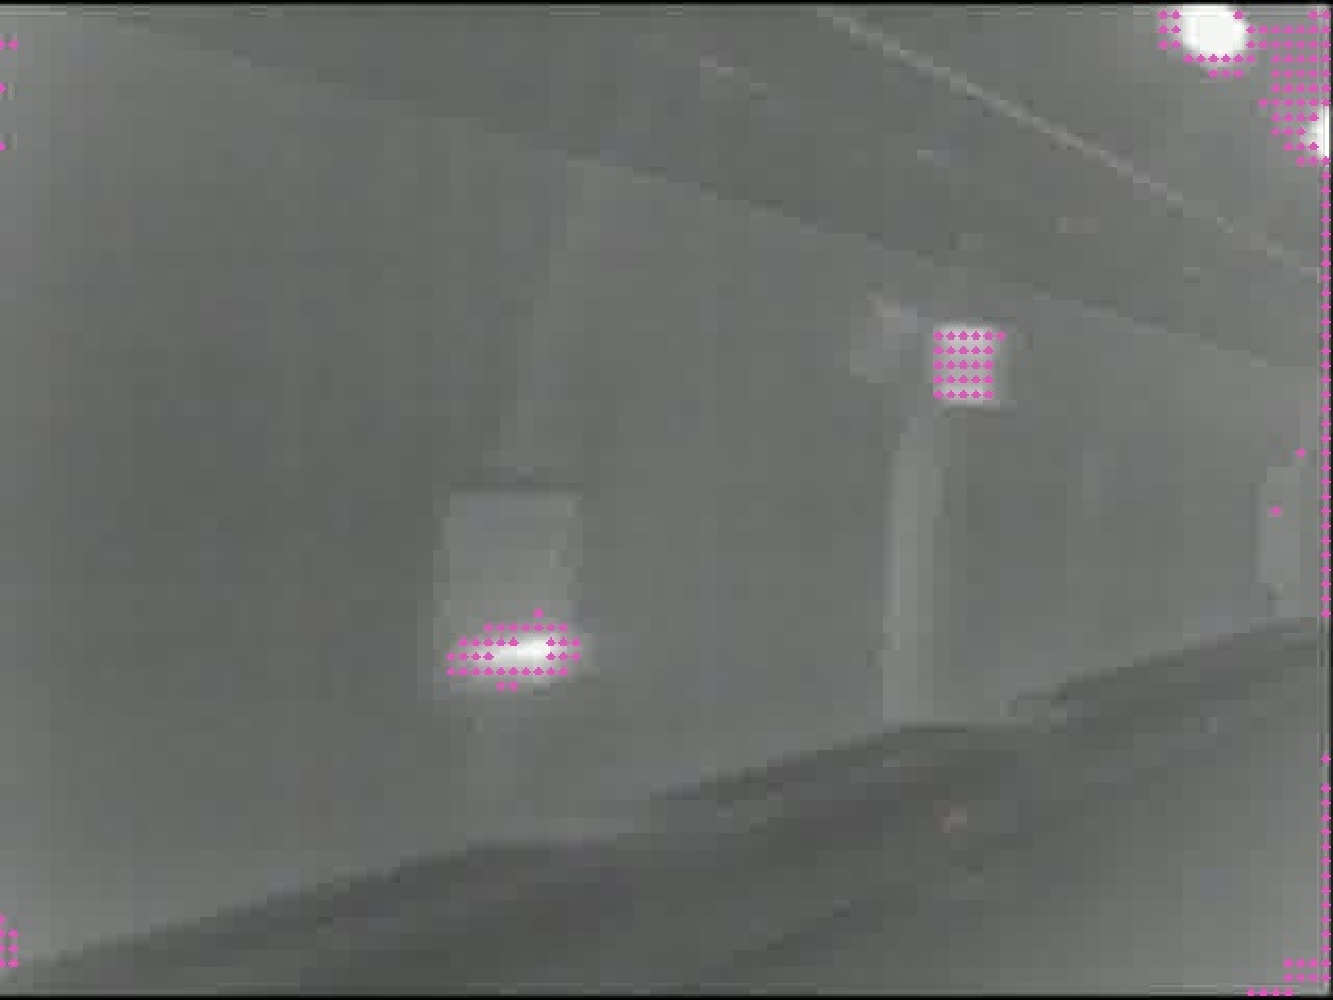
\includegraphics[width=0.22\textwidth,bb=0 0 640 480]{8Kptimg00028.ps}
\label{fig:sec:b}}
\caption{Keypoint detection. }
\label{fig:sec}
\end{figure}
\subsection{Keypoint Verification}
As shown in Figure \ref{fig:sec:b}, the detected keypoints don't just belong to emergency telephone indicators, but also belong to the background. For training purposes, keypoints belonging to emergency telephone indicators are considered  positive, all others are negative.

To verify the keypoints, the appearance of the sub-image around each keypoint is used. Intensity histograms are used to describe the appearance. Noisy keypoints not only come from the wall of the tunnel, but also from ordinary lights, other vehicles, and other vehicles' shadows. Thus robust linear classifiers are not suitable for the verification. Here, a general model in the form of a simple mixture is used. The \emph{k}-means method is used to cluster the intensity histograms, $\{A_{\bf{x}},l_{\bf{x}}=1\}$, of the positive keypoints, and, $\{A_{\bf{x}},l_{\bf{x}}=0\}$,  of
the negative keypoints.

Let $\{C_1^i,i=1,2,...,n_1\}$ denote the intensity histogram centers of the positive keypoints, and $\{C_0^i,i=1,2,...,n_2\}$ the negative. For each $C_1$, the average Euclidean distance between $\{C_0^i,i=1,2,...,n_2\}$ is calculated as,
\begin{equation}
Eu(C_1^i)={\frac 1 n_2}\sum\limits^{n_2}_{j=1}Euclid(C_1^i,C_0^j)\;.
\label{eq2}
\end{equation}
Here, $Euclid(\cdot)$ calculates the Euclidean distance, and $Eu(\cdot)$ is an evaluation function of the positive feature centers. The positive feature centers are ranked by $Eu(\cdot)$, and the 10 positive feature centers with the largest $Eu(\cdot)$ are chosen and used for verification.

For verification, the intensity histogram of each keypoint's surrounding sub-image is extracted. Then the Euclidean distance between the extracted intensity histogram and its nearest positive feature center is calculated. If this distance exceeds a threshold, $D^{th}_{A_{\bf{x}}}$, it is considered negative, otherwise it is considered positive. Here, for simplicity, unlike~\cite{ac33}, the same threshold is used for all components of the mixture.

\begin{figure}
\centering
\subfigure[]{
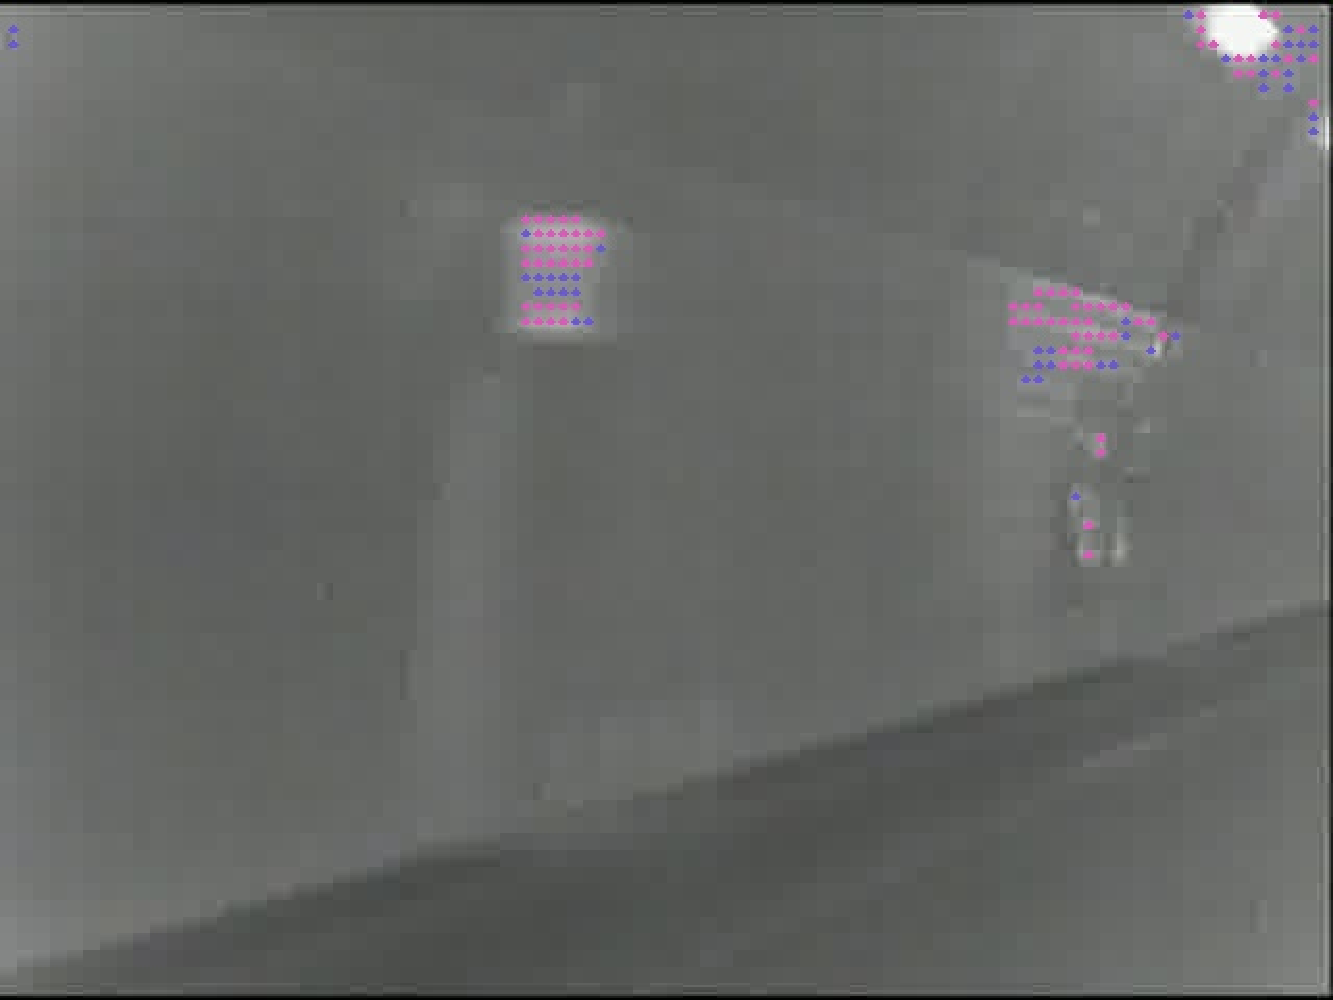
\includegraphics[width=0.22\textwidth,bb=0 0 640 480]{17VeriKptimg00039.ps}
\label{fig:thir:a}}
\subfigure[]{
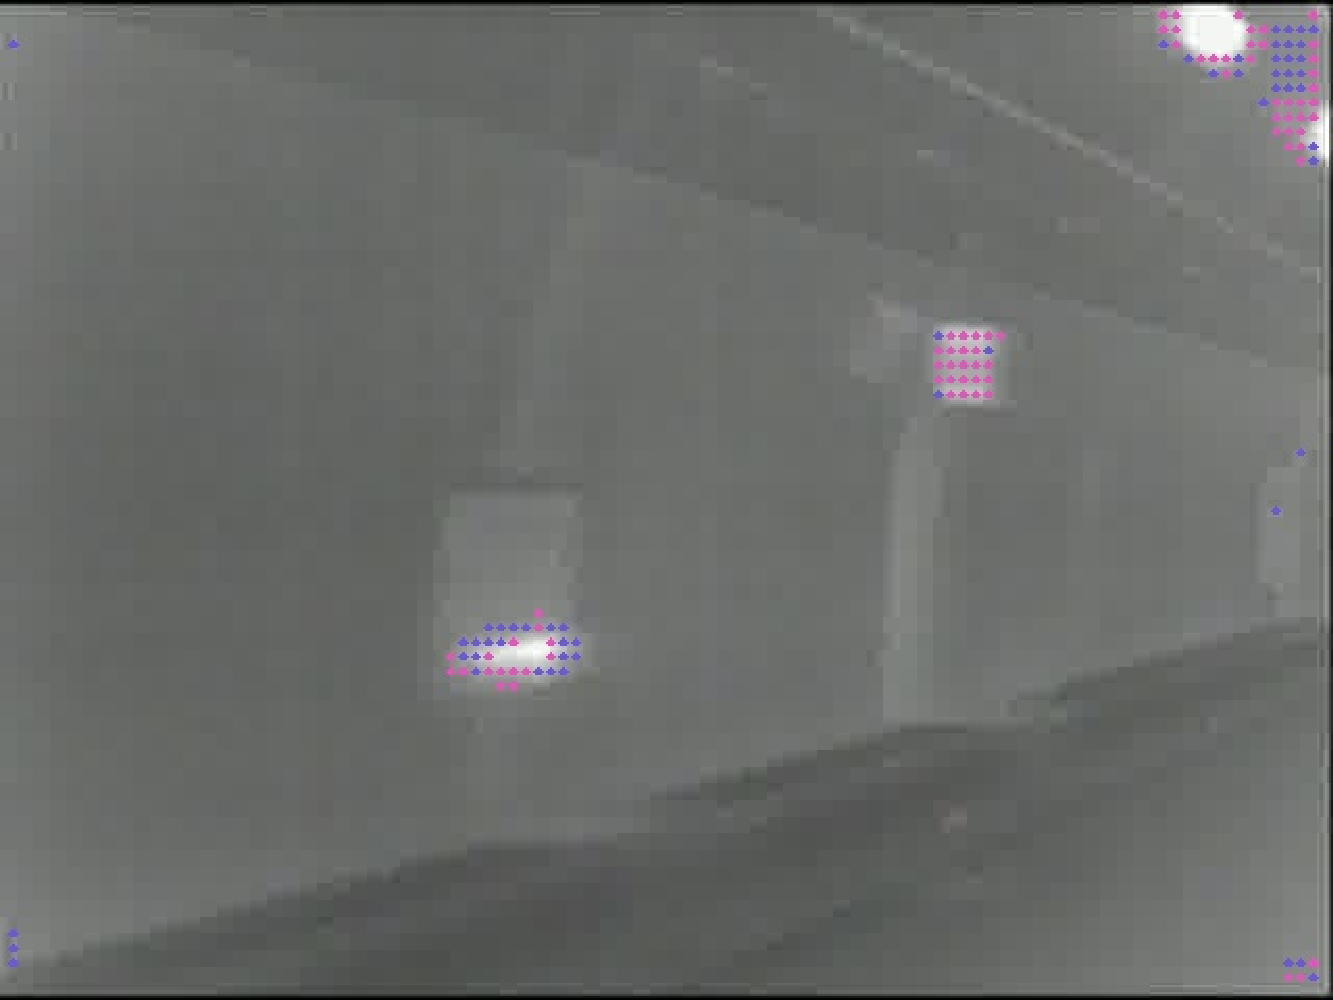
\includegraphics[width=0.22\textwidth,bb=0 0 640 480]{8VeriKptimg00028.ps}
\label{fig:thir:b}}
\subfigure[]{
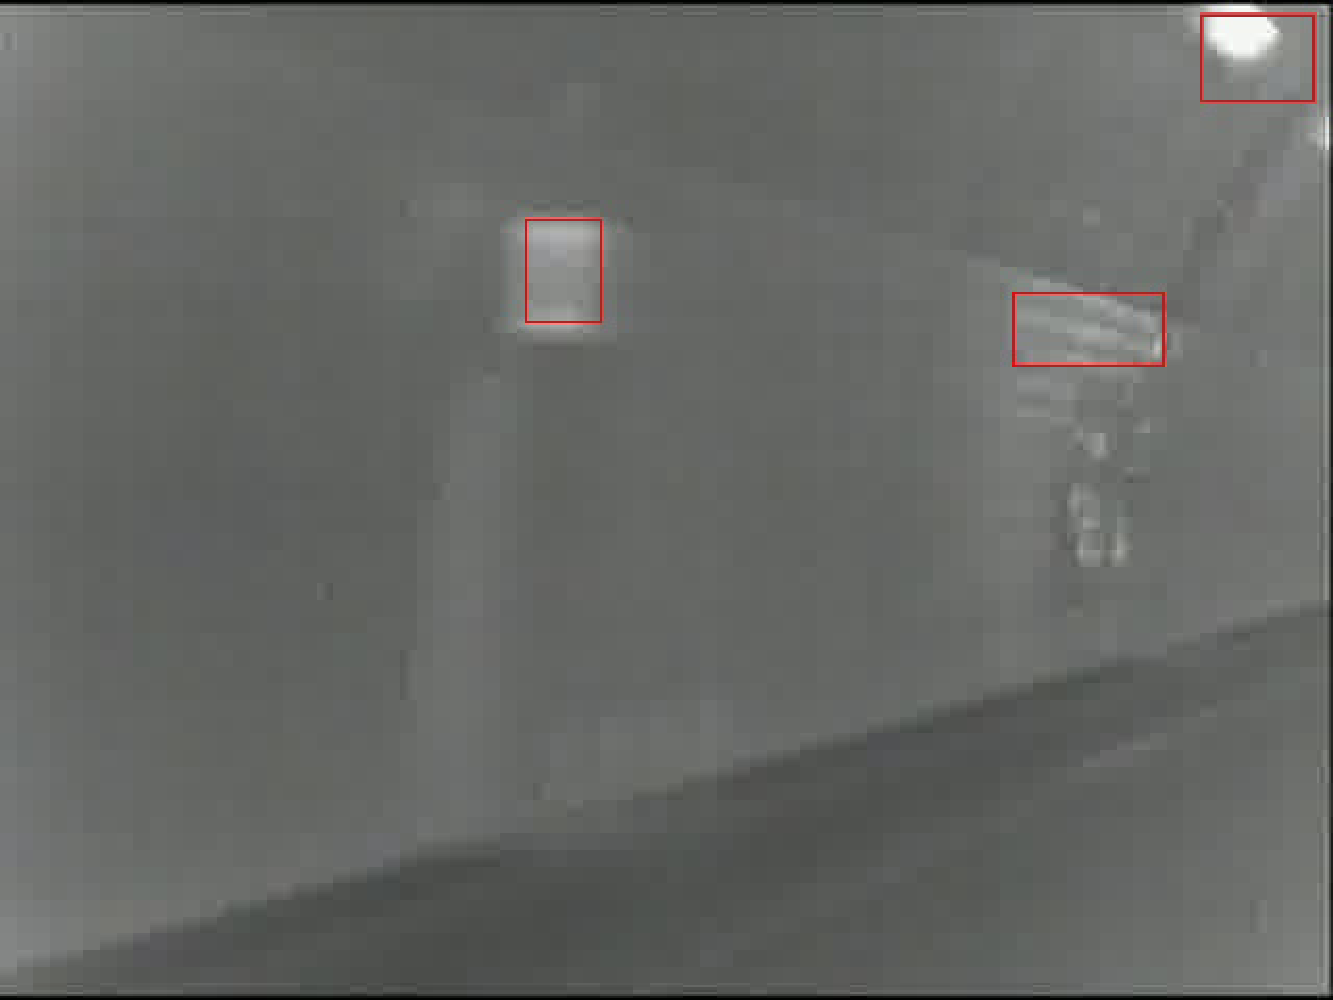
\includegraphics[width=0.22\textwidth,bb=0 0 640 480]{17Rgsimgwl00039.ps}
\label{fig:thir:c}}
\subfigure[]{
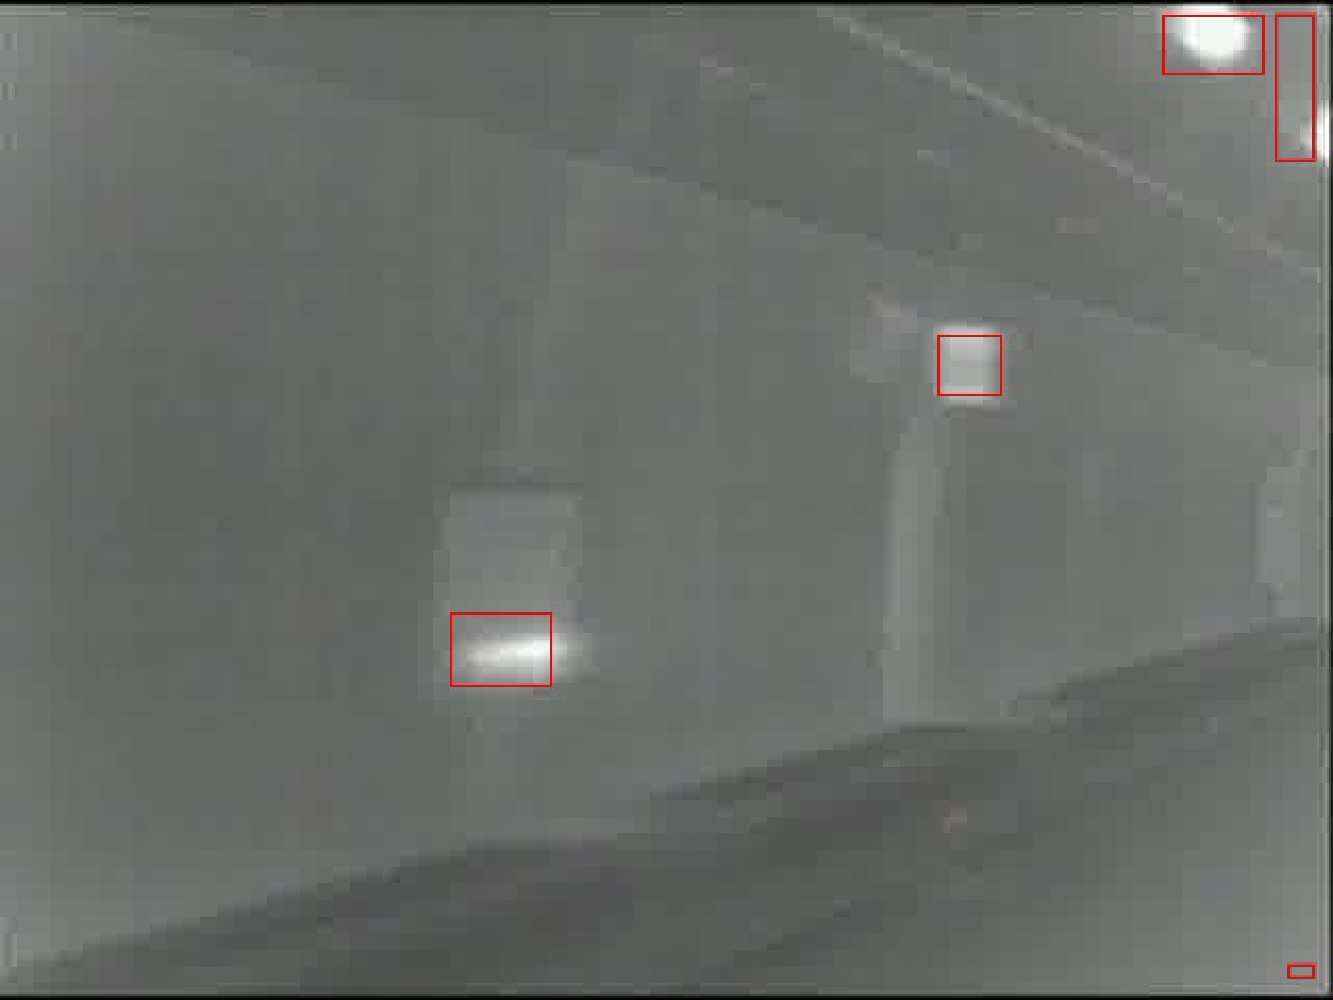
\includegraphics[width=0.22\textwidth,bb=0 0 640 480]{8Rgsimgwl00028.ps}
\label{fig:thir:d}}
\caption{Keypoint verification and clustering. Red circles mark keypoints which pass the verification, while blue marks failed ones. Rectangles mark keypoint clustering results. }
\label{fig:thir}
\end{figure}
\subsection{Keypoint Clustering}
After the keypoint verification step, on some frames the result is pretty good, while on other frames appearance of the keypoints is not enough to decide whether the keypoints belong to the emergency telephone indicators or not. Here generation of keypoint trajectories is not feasible, since nearby keypoints are similar in appearance and  the time complexity of associating such a large number of keypoints along the time dimension is high. So the keypoints are clustered, then data association in time dimension only is needed to deal with a small number of keypoint clusters.

To cluster the keypoints, a minimum spanning tree (mst) is built using the pairwise Euclidean distance between two keypoints. Then the mst is split by cutting edges larger than a threshold. This results in a grouping  of the keypoints, denoted by, $\gamma=\{\bf{g}\}$.


\subsection{Keypoint Cluster Verification by Appearance}

For each keypoint cluster, the smallest bounding rectangle is considered a detection hypothesis, as shown in Figure \ref{fig:thir:c} and Figure \ref{fig:thir:d}. There are three main sources of noise: ordinary lights, other vehicles, and other vehicles' shadows. The global appearance of ordinary lights is different from that of the emergency telephone indicators'. As ordinary lights get further from the infrared camera, the intensities of their corresponding sub-images in the collected data gets lower. At a certain distance, the intensities of the ordinary lights are almost the same as the intensities of the emergency telephone indicators'. For ordinary lights of which the intensities are higher than the intensities of emergency telephone indicators', the transition regions from the lights to tunnel walls will have similar intensities as the emergency telephone indicators'.
This indicates that although locally the emergency telephone indicators share the same appearance with ordinary lights, globally they can still be distinguished by appearance. As for other vehicles and their shadows, their intensity range is very close to the intensity range of the emergency telephone indicators', and they can hardly be distinguished by appearance alone.



At this step, the keypoint clusters are verified by their appearance, ideally excluding keypoint clusters belonging to ordinary lights. An Adaboost machine is trained using intensity histograms of the emergency telephone indicators and ordinary lights. The appearance of other vehicles is close to that of the emergency telephone indicators, and they are not used for training the machine. For training of the machine, labeled 32-dimensional intensity histograms are firstly normalized. Then each weak classifier of the machine makes a decision on one dimension of the intensity histograms. After this step, each keypoint cluster is either labeled as positive or negative.

In this step, to emphasize the Adaboost machine's performance on the positive training examples, we set the initial weights of the positive training examples 7 times as large as the weights of the negative training examples.  Since in practice, whether each keypoint cluster is a target object or not is decided by both appearance and motion information. The difficulties of excluding noisy objects can be left for later steps.
\begin{figure}[b]
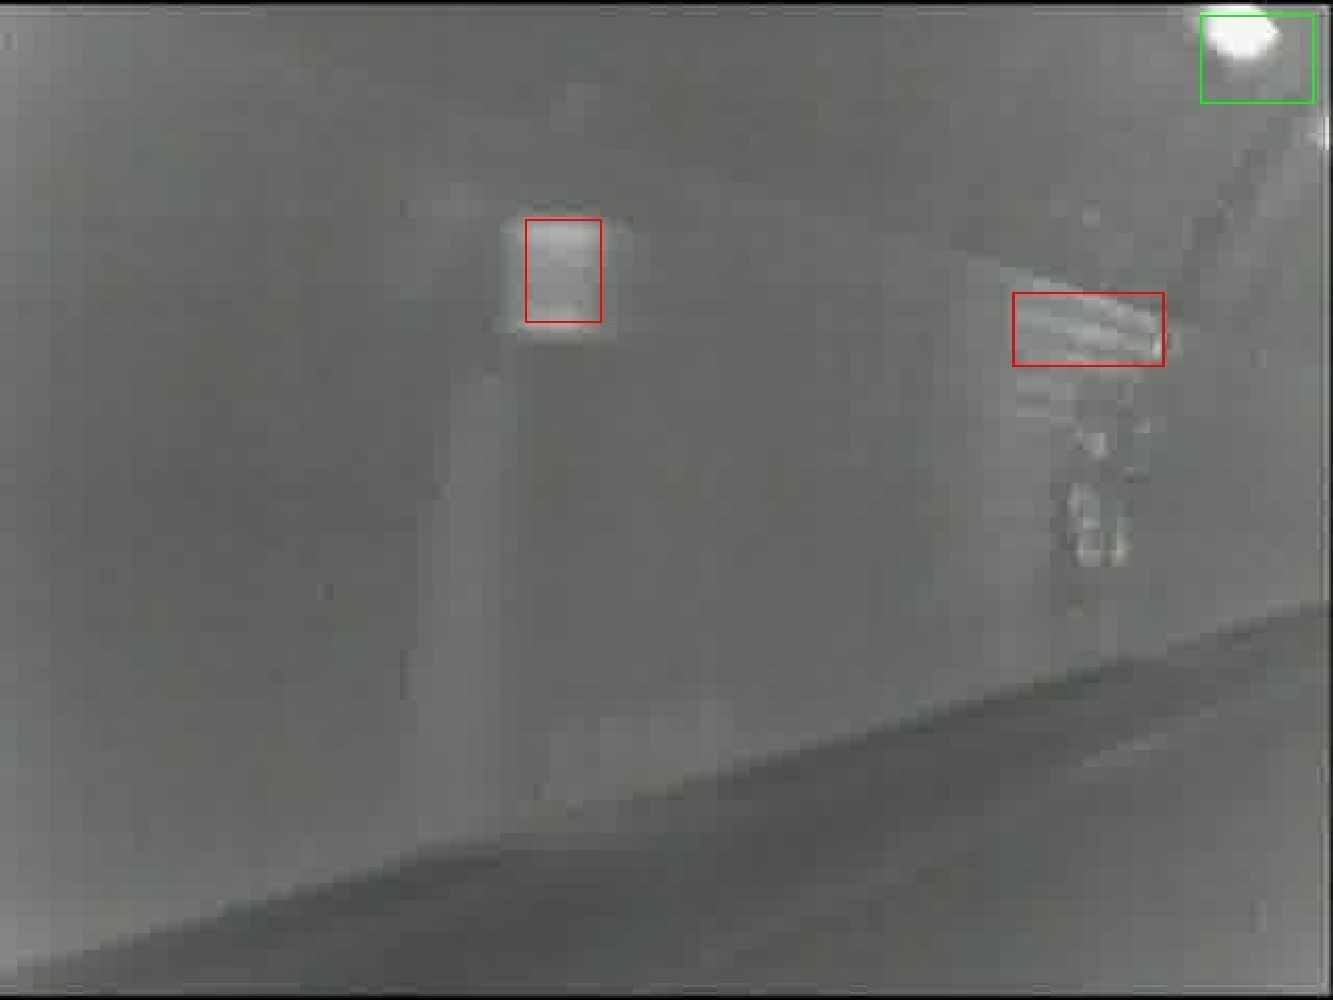
\includegraphics[width=0.22\textwidth,bb=0 0 640 480]{17Rgsimg00039.ps}
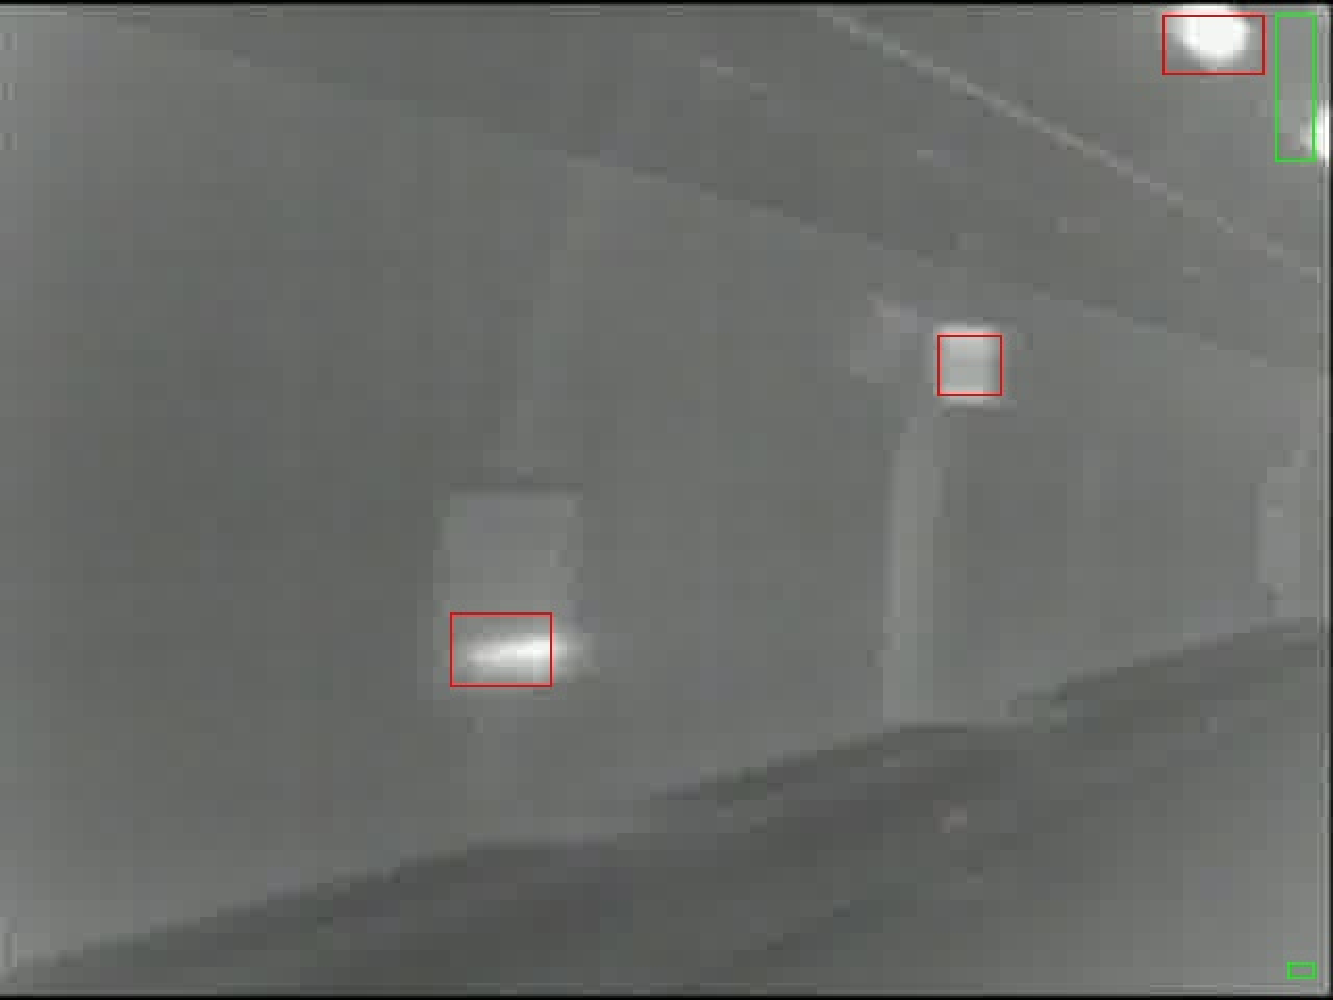
\includegraphics[width=0.22\textwidth,bb=0 0 640 480]{8Rgsimg00028.ps}
\caption{Keypoint cluster verification by appearance. Red rectangles: positive detection hypotheses, and green: negative detection hypotheses.}
\label{fig:fif}
\end{figure}
\subsection{Keypoint Cluster Tracking}
Not all noisy detection hypotheses can be excluded by using appearance, as shown in Figure \ref{fig:fif}. To distinguish keypoint clusters belonging to other vehicles and their shadows, the keypoint clusters are tracked through frames to generate trajectories.

In our case of keypoint cluster tracking, the problem is relatively simple, since no occlusion occurs. To keep the method on-line and maintain efficiency, a pool of trajectories are kept, $\tau=\{T_{\bf{g}}^i,i=1,2,...,n\}$, and new detection hypotheses act as detection responses, $\nu=\{n_{\bf{g}}^i,i=1,2,...m\}$, in tracking. The problem of tracking is modeled by finding the best data association hypothesis, $H^*$, between the trajectory set and detection response set as,
\begin{equation}
\begin{aligned}
{H^*} &= \mathop {\arg \max }\limits_{H \in \eta
} (P(H|\tau,\nu )) \\
&= \mathop {\arg \max }\limits_{H \in \eta }
(\prod\limits_{(T_{\bf{g}}^i,n_{\bf{g}}^j) \in H} {P_{link}(n_{\bf{g}}^j|T_{\bf{g}}^i)} ) \;.
\end{aligned}
\label{eq3}
\end{equation}
Let $u_{ij}=1 \mbox{ or } 0$ indicate if $n_{\bf{g}}^j$ is linked to $T_{\bf{g}}^i$ or not, and assuming each trajectory can link once, and each detection response can only be linked once, the problem can be modeled as,
\[
\begin{aligned}
&\arg \max\limits_{u_{ij}} \sum\limits_{i = 1}^n \sum\limits_{j = 1}^m u_{ij} \ln P_{link}(n_{\bf{g}}^j|T_{\bf{g}}^i)\\
&
\begin{aligned}
    s.t.:\mbox{ }&u_{ij}=0\mbox{ or }u_{ij}=1,\forall\;i,\forall\;j;\\
    &\sum\limits_{i = 1}^n {u_{ij}} \leq 1\;; \sum\limits_{j = 1}^m {u_{ij}}\leq 1\;.
\end{aligned}
\end{aligned}
\]
Here, $P_{link}(n_{\bf{g}}^j|T_{\bf{g}}^i)$ is defined by the appearance difference, the scale difference, and the time gap between the last detection response contained in $T_{\bf{g}}^i$ and $n_{\bf{g}}^j$. While the Hungarian algorithm~\cite{ha} gives a near-optimal solution, we follow a very simple manner for the solution by finding the best matched pairs and excluding them until no matching pairs can be found.

\subsection{Keypoint Cluster Verification by Motion}
As shown in Figure \ref{fig:sixs}, the trajectories from keypoint clusters belonging to emergency telephone indicators are different from other objects' trajectories. In this step, the temporal information encoded in the trajectories is used to further verify the keypoint clusters. A linear model is used to fit each trajectory, and the Pearson Correlation Coefficient(PCC) of the fitting is the criteria for the decision. Let $(x^i_{\bf{g}},y^i_{\bf{g}})$ denote the coordinate of the $i$th element belonging to a trajectory. The linear assumption is that $y^i_{\bf{g}}=a_0+a_1{x^i_{\bf{g}}}$. The PCC of the fitting is defined as,
\begin{equation}
r =| \frac{{\sum\limits_i {\left( {{x^i_{\bf{g}}} -  {\bar x_{\bf{g}}}} \right)\left( {{y^i_{\bf{g}}} -  {\bar y_{\bf{g}}}} \right)} }}{{{{\left[ {\sum\limits_i {{{\left( {{x^i_{\bf{g}}} -  {\bar x_{\bf{g}}}} \right)}^2} \cdot \sum\limits_i {{{\left( {{y^i_{\bf{g}}} -  {\bar y_{\bf{g}}}} \right)}^2}} } } \right]}^{1/2}}}}|\;.
\label{eq4}
\end{equation}
Where $r$ is used to decide if the trajectories of the keypoint clusters belong to emergency telephone indicators or not.
\subsection{Object Detection}
For each keypoint cluster on the current frame, there exists a label given by the Adaboost machine according to its appearance, and the likelihood of fitting its trajectory to a straight line.  For each keypoint cluster, it is considered an emergency telephone indicator if and only if its label - given by the Adaboost machine - is positive, its trajectory is longer than $l^{th}$, and the likelihood of fitting its trajectory to a straight line is larger than $r^{th}$.

Each trajectory not only connects the detection responses, but also connects the decisions for detection responses made by their appearance and motion patterns. The target objects and noisy objects actually appear in successive frames, and even if we make a wrong decision on one frame, we can expect to recover from this mistake based on the results of other frames. The final results are based on the trajectories of decisions. When one trajectory ends, if more than 80\% of the decisions it connects are positive, then this trajectory is considered positive.




\section{Experimental Results}
We evaluate our method based on detection performance and efficiency.

\textbf{Data} To collect data, we mount an infrared camera on top of the experimental vehicle, and then  take several tours of the Awagatake tunnel. Approximately 7,000 frames are collected for each tour. The frame size is $640\times 480$, the intensity range is [0,255], and the frame rate is 30 frames per second.

\textbf{Implementation Settings} All models are trained using data from the same tour, while evaluated using data from another tour.

To set intensity thresholds for keypoint detection, Gaussian distribution is assumed for the points belonging to emergency telephone indicators. Following the $3\sigma$ principle, $I^{th1}_{\bf{x}}$ is set to 160 and $I^{th2}_{\bf{x}}$ to 190.
The approximate sub-images of the emergency telephone indicators are manually marked, and used for training the mixture model of keypoint verification. The detected keypoints falling into the sub-image are marked as positive, all other points are marked negative. Note that this model and the training method may not be very accurate, since more accurate marking requires more manual effort. About 30,000 intensity histograms of the positive keypoints are sampled, and about 3,000,000 of the negative. When using of $k$-means for clustering the positive intensity histograms, $k$ is set to 40; it is set to 400 for the negative. By using these $k$ values,  both feature sets are over-segmented. The threshold to verify keypoints $D^{th}_{A_{\bf{x}}}$ is set to 0.14 for the normalized histograms.
For keypoint clustering, the threshold to split the mst is set to 40, which is half the largest height of the emergency telephone indicators.
The Adaboost machine used to distinguish other vehicles and their shadows is trained by intensity histograms of positive keypoint clusters and negative keypoint clusters. We manually mark  positive  and  negative keypoint clusters. If the Adaboost machine is trained by averagely weighted training examples, its correct rate on the training examples is overall 84\%. When trained using our bias weighted training examples, its correct rate is  94\% for the positive training examples, and 77\% for the negative training examples.
During keypoint cluster tracking, whether a detection response can be linked to a trajectory or not is constrained by position and scale changes. Here scale change limit is set to 4. When the trajectories are fitted as lines, the linear model is also used in associating new detection responses.



\begin{figure}
{
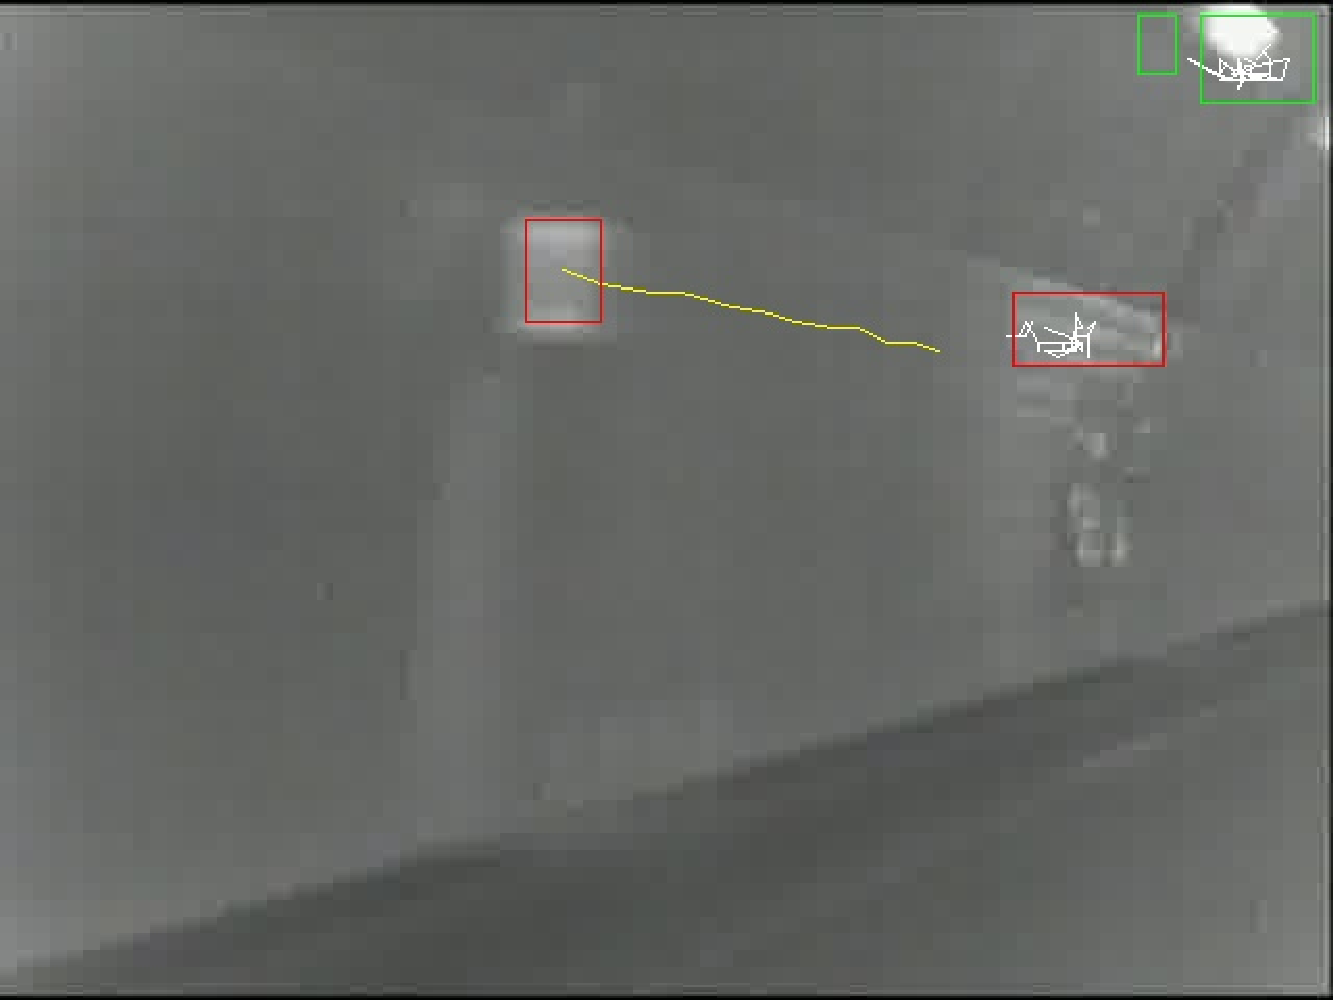
\includegraphics[width=0.22\textwidth,bb=0 0 640 480]{17veriTrjimg00039.ps}
}
{
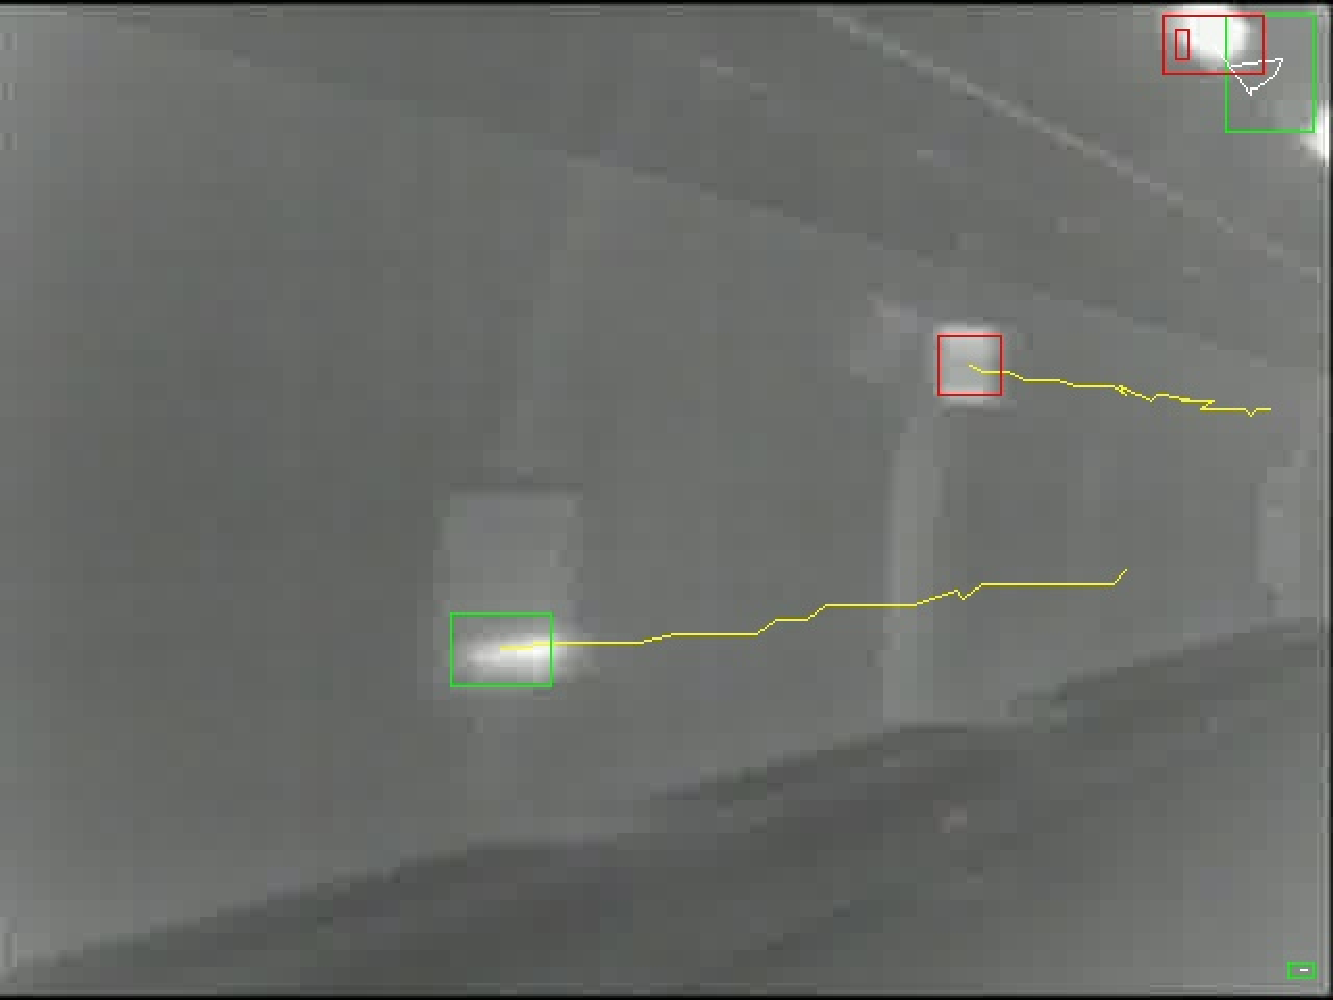
\includegraphics[width=0.22\textwidth,bb=0 0 640 480]{8veriTrjimg00028.ps}
}\\
{
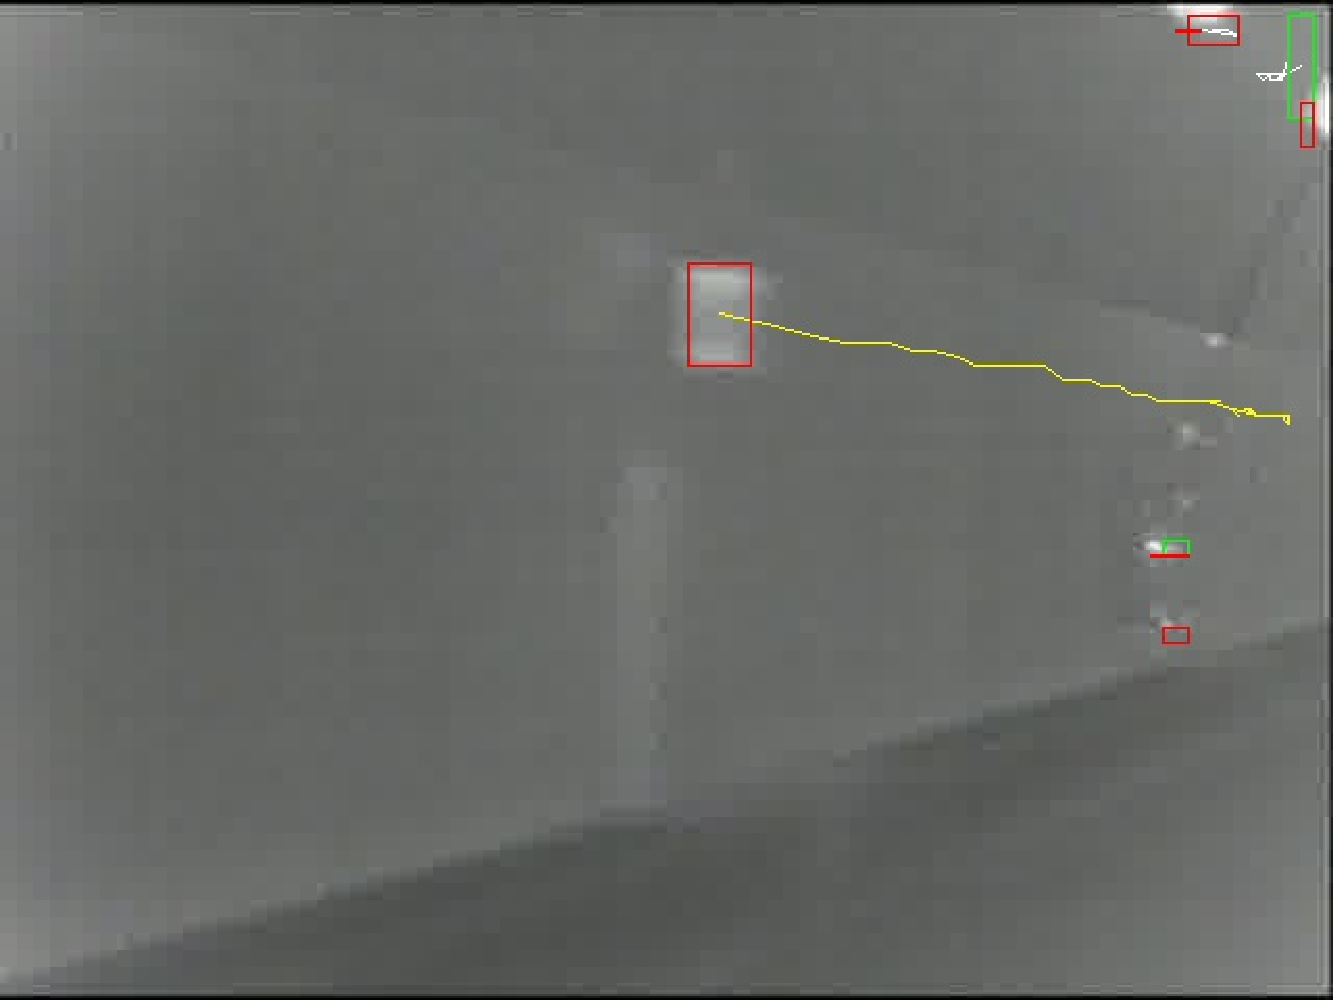
\includegraphics[width=0.22\textwidth,bb=0 0 640 480]{19veriTrjimg00041.ps}
}
{
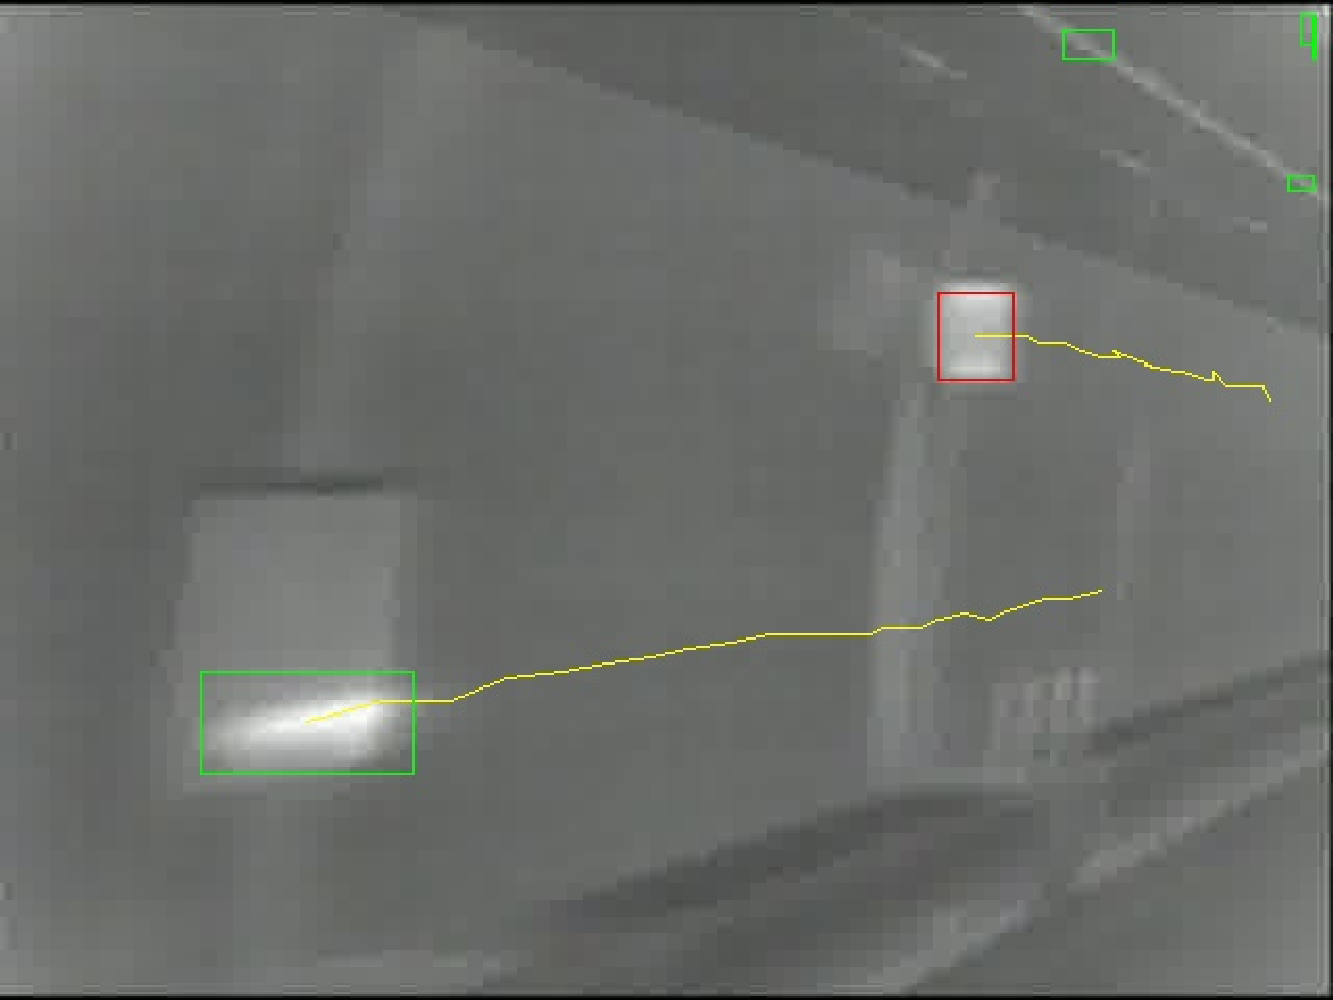
\includegraphics[width=0.22\textwidth,bb=0 0 640 480]{3veriTrjimg00023.ps}
}
\caption{Detection results.}
\label{fig:sixs}
\end{figure}

\textbf{Detection Results}

Using an ordinary desktop computer with Intel Core2 Quad 2.6GHz processors, the method deals with real data at a frame rate of 41 frames per second, and this fulfills real-time requirements.


The detection rate and false alarm rate are evaluated on the keypoint clusters as shown in TABLE \ref{tb:tb2}.
More detection results are shown in Figure \ref{fig:sixs}.
\begin{table}[h]
\centering
\begin{tabular}{lll}
     \hline
     \hline
    total number &	472 + 3304  \\
    correctly labeled &	468   \\
    miss detections &	4 &	  \\
    false alarms &	22    \\
    detection rate &	99.2\% &	  \\
    false alarm rate &	0.7\% &	   \\
   \hline
\end{tabular}
\caption{Detection rate and false alarm rate.}\label{tb:tb2}
\end{table}

While evaluated on a much smaller dataset, the detection rate and false alarm rate of~\cite{wang1} are 90\% and 19\% respectively. Our experiment outperforms~\cite{wang1}, because our sensed images are much clearer, and also because of our more effective training of the Adaboost machine.

The results on the trajectories of decisions are also evaluated. The method correctly detects all of the 22 emergency telephone indicators with no false alarms. The detection rate is 100\%, and the false alarm rate is 0\%.

\section{Conclusion}
We propose an object detection method to detect emergency telephone indicators in a tunnel environment. The method makes use of appearance and motion information of the target objects in a hierarchical manner. With careful optimization of the detection pipeline, the method gives promising results in real time. Based on the detection results, a positioning system in a tunnel environment can be expected.


% conference papers do not normally have an appendix


% use section* for acknowledgement
\section*{Acknowledgment}


The work is in part supported by NEDO. The first author is sponsored by China Scholarship Council. The authors thank Patricia Knapp and Kent Fujiwara for revising suggestions on the manuscript.




{\small
\bibliographystyle{ieee}
\bibliography{egbib}
}









\end{document}
